%%%%%%%%%%%%%%%%%%%%%%%%%%%%%%%%%%%%%%%%%%%%%%%%%%%%%%%%%%%%%%%%%%%%%%%%%%%%%%%%
%% Plantilla de memoria en LaTeX para la EIF - Universidad Rey Juan Carlos
%%
%% Por Gregorio Robles <grex arroba gsyc.urjc.es>
%%     Grupo de Sistemas y Comunicaciones
%%     Escuela de Ingeniería de Fuenlabrada
%%     Universidad Rey Juan Carlos
%% (muchas ideas tomadas de Internet, colegas del GSyC, antiguos alumnos...
%%  etc. Muchas gracias a todos)
%%
%% La última versión de esta plantilla está siempre disponible en:
%%     https://github.com/gregoriorobles/plantilla-memoria
%%
%% Para obtener PDF, ejecuta en la shell:
%%   make
%% (las imágenes deben ir en PNG o JPG)

%%%%%%%%%%%%%%%%%%%%%%%%%%%%%%%%%%%%%%%%%%%%%%%%%%%%%%%%%%%%%%%%%%%%%%%%%%%%%%%%

\documentclass[a4paper, 12pt]{book}
%\usepackage[T1]{fontenc}

\usepackage[a4paper, left=2.5cm, right=2.5cm, top=3cm, bottom=3cm]{geometry}
\usepackage{times}
\usepackage[utf8]{inputenc}
\usepackage[spanish]{babel} % Comenta esta línea si tu memoria es en inglés
\usepackage{url}
%\usepackage[dvipdfm]{graphicx}
\usepackage{graphicx}
\usepackage{float}  %% H para posicionar figuras
\usepackage[nottoc, notlot, notlof, notindex]{tocbibind} %% Opciones de índice
\usepackage{latexsym}  %% Logo LaTeX

\title{Memoria del Proyecto}
\author{Nombre del autor}

\renewcommand{\baselinestretch}{1.5}  %% Interlineado

\begin{document}

\renewcommand{\refname}{Bibliografía}  %% Renombrando
\renewcommand{\appendixname}{Apéndice}


%%%%%%%%%%%%%%%%%%%%%%%%%%%%%%%%%%%%%%%%%%%%%%%%%%%%%%%%%%%%%%%%%%%%%%%%%%%%%%%%
% PORTADA

\begin{titlepage}
\begin{center}

\includegraphics[scale=0.6]{img/URJ_logo_Color_POS.png}

\vspace{1.75cm}

\LARGE
ESCUELA DE INGENIERÍA DE FUENLABRADA
\vspace{1cm}

\LARGE
GRADO EN INGENIERÍA DE TECNOLOGÍAS DE TELECOMUNICACIÓN

\vspace{1cm}
\LARGE
\textbf{TRABAJO FIN DE GRADO}

\vspace{2cm}

\Large
EVOLUCIÓN DE LA PARTICIPACIÓN VOLUNTARIA DE PROYECTOS DE SOFTWARE LIBRE:
EVIDENCIAS DE DEBIAN

\vspace{2cm}

\large
Autor : Pablo Cabeza Portalo \\
Tutor : Dr. Gregorio Robles\\

\vspace{1cm}

\large
Curso académico 2023/2024

\end{center}
\end{titlepage}

\newpage
\mbox{}
\thispagestyle{empty} % para que no se numere esta pagina



%%%%%%%%%%%%%%%%%%%%%%%%%%%%%%%%%%%%%%%%%%%%%%%%%%%%%%%%%%%%%%%%%%%%%%%%%%%%%%%%
%%%% Para firmar
\clearpage
\pagenumbering{gobble}
\chapter*{}

\vspace{-4cm}
\begin{center}
\LARGE
\textbf{Trabajo Fin de Grado}

\vspace{1cm}
\large
Evolución de la Participación Voluntaria en Proyectos de Software Libre:
Evidencia de Debian

\vspace{1cm}
\large
\textbf{Autor :} Pablo Cabeza Portalo \\
\textbf{Tutor :} Dr. Gregorio Robles

\end{center}

\vspace{1cm}
La defensa del presente Proyecto Fin de Carrera se realizó el día \qquad$\;\,$ de \qquad\qquad\qquad\qquad \newline de 2024, siendo calificada por el siguiente tribunal:


\vspace{0.5cm}
\textbf{Presidente:}

\vspace{1.2cm}
\textbf{Secretario:}

\vspace{1.2cm}
\textbf{Vocal:}


\vspace{1.2cm}
y habiendo obtenido la siguiente calificación:

\vspace{1cm}
\textbf{Calificación:}


\vspace{1cm}
\begin{flushright}
Fuenlabrada, a \qquad$\;\,$ de \qquad\qquad\qquad\qquad de 2024
\end{flushright}

%%%%%%%%%%%%%%%%%%%%%%%%%%%%%%%%%%%%%%%%%%%%%%%%%%%%%%%%%%%%%%%%%%%%%%%%%%%%%%%%
%%%% Dedicatoria

\chapter*{}
\pagenumbering{Roman} % para comenzar la numeracion de paginas en numeros romanos
\begin{flushright}
\textit{Dedicado a \\
mi familia, mis amigos y a mi pareja.}
\end{flushright}

%%%%%%%%%%%%%%%%%%%%%%%%%%%%%%%%%%%%%%%%%%%%%%%%%%%%%%%%%%%%%%%%%%%%%%%%%%%%%%%%
%%%% Agradecimientos

\chapter*{Agradecimientos}
%\addcontentsline{toc}{chapter}{Agradecimientos} % si queremos que aparezca en el índice
\markboth{AGRADECIMIENTOS}{AGRADECIMIENTOS} % encabezado 

Este es el fin de una de las etapas más importantes de mi vida y por ello quiero agradecer a varias personas que me han acompañado en este proceso.
Primero quiero agradecer a mi madre Antonia todo el apoyo que me ha dado en cada una de mis decisiones, tanto personales como académicas. Eres quien me impulsa a lograr mis sueños.
Segundo a mi padre Manuel que siempre ha sido mi ejemplo a seguir. Me ha aportado valores fundamentales como el trabajo y el esfuerzo que han sido imprescindibles para abordar esta carrera.
Gracias a los dos por darme la vida.
También agradecer a mi tutor, Gregorio, por darme este proyecto, tener paciencia  y ayudarme en todo cuanto pudo para desarrollarlo.
Por último, quiero agradecer a esa persona tan especial que conocí en esta universidad y que me dio la confianza y la fuerza necesaria para lograr mis metas. 
Paula, gracias por ser mi compañera de viaje y por aparecer en el momento que mas lo necesitaba. Hemos afrontado este desafío juntos y sin ti no hubiera sido igual.


%%%%%%%%%%%%%%%%%%%%%%%%%%%%%%%%%%%%%%%%%%%%%%%%%%%%%%%%%%%%%%%%%%%%%%%%%%%%%%%%
%%%% Resumen

\chapter*{Resumen}
%\addcontentsline{toc}{chapter}{Resumen} % si queremos que aparezca en el índice
\markboth{RESUMEN}{RESUMEN} % encabezado

Aquí viene un resumen del proyecto.
Ha de constar de tres o cuatro párrafos, donde se presente de manera clara y concisa de qué va el proyecto. 
Han de quedar respondidas las siguientes preguntas:

\begin{itemize}
  \item ¿De qué va este proyecto? ¿Cuál es su objetivo principal?
  \item ¿Cómo se ha realizado? ¿Qué tecnologías están involucradas?
  \item ¿En qué contexto se ha realizado el proyecto? ¿Es un proyecto dentro de un marco general?
\end{itemize}

Lo mejor es escribir el resumen al final.

%%%%%%%%%%%%%%%%%%%%%%%%%%%%%%%%%%%%%%%%%%%%%%%%%%%%%%%%%%%%%%%%%%%%%%%%%%%%%%%%
%%%% Resumen en inglés

\chapter*{Summary}
%\addcontentsline{toc}{chapter}{Summary} % si queremos que aparezca en el índice
\markboth{SUMMARY}{SUMMARY} % encabezado

Here comes a translation of the ``Resumen'' into English. 
Please, double check it for correct grammar and spelling.
As it is the translation of the ``Resumen'', which is supposed to be written at the end, this as well should be filled out just before submitting.


%%%%%%%%%%%%%%%%%%%%%%%%%%%%%%%%%%%%%%%%%%%%%%%%%%%%%%%%%%%%%%%%%%%%%%%%%%%%%%%%
%%%%%%%%%%%%%%%%%%%%%%%%%%%%%%%%%%%%%%%%%%%%%%%%%%%%%%%%%%%%%%%%%%%%%%%%%%%%%%%%
% ÍNDICES %
%%%%%%%%%%%%%%%%%%%%%%%%%%%%%%%%%%%%%%%%%%%%%%%%%%%%%%%%%%%%%%%%%%%%%%%%%%%%%%%%

% Las buenas noticias es que los índices se generan automáticamente.
% Lo único que tienes que hacer es elegir cuáles quieren que se generen,
% y comentar/descomentar esa instrucción de LaTeX.

%%%% Índice de contenidos
\tableofcontents 
%%%% Índice de figuras
\cleardoublepage
%\addcontentsline{toc}{chapter}{Lista de figuras} % para que aparezca en el indice de contenidos
\listoffigures % indice de figuras
%%%% Índice de tablas
%\cleardoublepage
%\addcontentsline{toc}{chapter}{Lista de tablas} % para que aparezca en el indice de contenidos
%\listoftables % indice de tablas


%%%%%%%%%%%%%%%%%%%%%%%%%%%%%%%%%%%%%%%%%%%%%%%%%%%%%%%%%%%%%%%%%%%%%%%%%%%%%%%%
%%%%%%%%%%%%%%%%%%%%%%%%%%%%%%%%%%%%%%%%%%%%%%%%%%%%%%%%%%%%%%%%%%%%%%%%%%%%%%%%
% INTRODUCCIÓN %
%%%%%%%%%%%%%%%%%%%%%%%%%%%%%%%%%%%%%%%%%%%%%%%%%%%%%%%%%%%%%%%%%%%%%%%%%%%%%%%%

\cleardoublepage
\chapter{Introducción}
\label{sec:intro} % etiqueta para poder referenciar luego en el texto con ~\ref{sec:intro}
\pagenumbering{arabic} % para empezar la numeración de página con números

Vivimos en un mundo totalmente digitalizado en el que la presencia de ordenadores está a la orden del día. Con esto no nos referimos únicamente a ordenadores de escritorio. A diario interactuamos con una amplia gama de dispositivos compuestos por ordenadores camuflados. Desde electrodomésticos inteligentes pasando por coches modernos hasta en tarjetas de crédito. Estos tienen incorporados ordenadores pequeños pero potentes que realizan una serie de tareas para el beneficio y la mejora de la vida humana.

En la mayoría de estos ordenadores de uso cotidiano, como portátiles o móviles, se aloja un Sistema Operativo. Un Sistema Operativo es el “intermediario” entre el usuario y el hardware del ordenador a partir de software. Gestiona los recursos del hardware proporcionando una interfaz al usuario. De esta forma pueden interactuar con dicho ordenador. 
Algunos de los sistemas operativos más usados son: iOS, Android, macOS, Microsoft Windows o Linux. 

Linux es un sistema operativo de código abierto el cual es gratuito para cualquier usuario que quiera adoptarlo en su computadora. Este consta de muchas distribuciones. Las distribuciones son versiones del Sistema Operativo de Linux desarrolladas por diferentes individuos, equipos o empresas para mejorar la experiencia de los usuarios.

Una de estas distribuciones es “Debian” y es sobre la que tratará este estudio.
Debian es un Sistema Operativo que trabaja con el Kernel (núcleo) de Linux y ha ido aportando distintas versiones desde 1993. 
Treinta años después nos preguntamos ciertas cosas como, ¿Los individuos que trabajaban en las primeras versiones siguen actualizando Debian? ¿Se trabaja individualmente o por equipos? ¿Cuántos paquetes sacan en cada versión? ¿Qué ocurre con ellos? Todo esto lo veremos a continuación.



\section{Contexto}
\label{sec:contexto}



\subsection{Proyecto Debian}
\label{subsec:proyecto debian}

El Proyecto Debian está formado por un grupo de voluntarios a nivel mundial que trabajan para producir una distribución del Sistema Operativo Linux basada en "software libre".

Con el término "software libre" no nos referimos a su coste. Este va enfocado a la "libertad real" dentro del software, es decir, "software de código abierto".
Esto significa que cualquier usuario puede acceder al código fuente para estudiarlo, revisarlo, modificarlo o distribuirlo sin restricción alguna.

Debian es la distribución de Linux más relevante sin fines comerciales.
En su comienzo, fue la única abierta a la participación de diferentes usuarios que quisieran aportar al proyecto con su trabajo.

Con el tiempo fue asentando un gran conjunto de directrices y procedimientos para el empaquetamiento y distribución de software. Esto les sirvió para poder alcanzar los estándares de calidad requeridos y con ello asegurar su buen funcionamiento.

\subsection{Versiones Debian}
\label{subsec:versiones debian}

Debian está conformado por varias versiones desde 1993 las cuales explicaremos a continuación:

\begin{itemize}

	\item \textbf {Versiones 0.x (1993 - 1995):} estas versiones fueron las primeras y mas rudimentarias pero dieron lugar a la creación de Debian gracias a su creador \textbf {Ian Murdock}.
	\begin{itemize}
		\item \textbf {Debian 0.01 hasta 0.90.}
		\item \textbf {Debian 0.91:} disponía de un sencillo sistema de empaquetamiento que permitía instalar y desinstalar paquetes.
		\item \textbf {Debian 0.93R5:}  se asignaron responsabilidades de cada paquete a cada uno de los desarrolladores. Se comenzo a usar el administrador de paquetes \textbf {dpkg} para la instalación de paquetes después de la instalación del sistema.
		base.
	\end{itemize}
	\item \textbf {Versiones 1.x (1996 - 1997):} \textbf{Bruce Perens} fue designado como líder del proyecto después de que Ian lo designara.
	\begin{itemize}
		\item \textbf {Debian 1.0:} esta versión nunca fue publicada debido a una confusión al distribuir una versión en desarrollo con el nombre equivocado de Debian 1.0 que daría problemas en ejecución.
		\item \textbf {Debian 1.1 Buzz: } es la primera versión de Debian con un nombre en clave sacado de las peliculas de \textbf {"Toy Story"}.
		\item \textbf {Debian 1.2 Rex: } esta versión estaba completamente en formato \textbf{ELF} y usaba el núcleo (kernel) Linux 2.0.
		
		El formato \textbf{ELF} (Executable and Linkable Format) es un estándar. Se usa en sistemas operativos tipo \textbf{UNIX} (como Linux). Sirve para organizar y manejar archivos ejecutables, bibliotecas compartidas y otros objetos binarios.
		\item \textbf {Debian 1.3 Bo}.
	\end{itemize}
	\item \textbf {Versiones 2.x (1998 - 2000):} \textbf{Ian Jackson} pasó a ser el líder del proyecto.
	\begin{itemize}
		\item \textbf {Debian 2.0 Hamm: }fue la primera versión multiplataforma de Debian. Agregó soporte para arquitecturas de la serie \textbf{Motorola 68000}.
		\item \textbf {Debian 2.2 Potato: }agregó soporte para las arquitecturas  PowerPC y ARM (CPU's de arquitectura RISC creadas por diferentes empresas).
	\end{itemize}
	\item \textbf {Versiones 3.x (2002 -2005):}
	\begin{itemize}
		\item \textbf {Debian 3.0 Woody: }se agregaron más arquitecturas a esta versión y fue la primera en usar \textbf {software criptográfico}. Este se usa para codificar información y mantener la transferencia segura de datos.
		\item \textbf {Debian 3.1 Sarge: }incluye un nuevo instalador llamado \textbf {debian-installer}. Contiene detección automática de hardware, instalación sin supervisión y está traducido a más de treinta idiomas.
	\end{itemize}
	\item \textbf {Debian 4.0 Etch (2007):}se añadieron mejoras como un instalador gráfico o la verificación criptográfica de los paquetes descargados entre otras.
	\item \textbf {Debian 5.0 Lenny (2009):}añadió la arquitectura \textbf {ARM EABI} para dar soporte a los nuevos procesadores \textbf {ARM}.
	\item \textbf {Debian 6.0 Squeeze: }con esta versión fue la primera vez que una distribución de Linux se extendía para permitir también el uso de un núcleo no Linux.
	\item \textbf {Debian 7.0 Wheezy (2011):}se introdujo el soporte de \textbf {multiarquitectura}. Esto permitía que los usuarios instalaran en una misma máquina paquetes de múltiples arquitecturas.
	\item \textbf {Debian 8 Jessie (2013):}trajo importantes mejoras de seguridad, como un nuevo kernel que solucionaba varias vulnerabilidades (como \textbf {ataques de enlace simbólico}).
	\item \textbf {Debian 9 Stretch (2015):}se introdujeron paquetes para la depuración a través de un repositorio nuevo en el archivo. Facilitaría el proceso de depuración y solución de problemas relacionados con esos paquetes.
	\item \textbf {Debian 10 Buster (2019):} incluyó por primera vez un marco de control de acceso obligatorio. Restringe las acciones que pueden realizar los programas, limitando su acceso a ciertos recursos del sistema, como archivos, directorios, redes, etc.
	\item \textbf {Debian 11 Bullseye (2021):} introduce un nuevo paquete, ipp-usb, que utiliza el protocolo IPP-over-USB, independiente del fabricante y soportado por muchas impresoras actuales. Esto permite que un dispositivo USB sea tratado como un dispositivo de red.
	
		
\end{itemize}
	


\section{Estructura de la memoria}
\label{sec:estructura}

A continuación se exponen los capítulos en los que se organiza esta memoria y los puntos clave tratados en cada uno de ellos:


\begin{itemize}
  \item \textbf {Capítulo 1: Introducción.} Se explica el contexto de Debian y las diferentes versiones distribuidas a lo largo de su historia.
  
  \item \textbf {Capítulo 2: Objetivos.} Se especifica cuales son los objetivos parciales para lograr el objetivo general.
  
  \item \textbf {Capítulo 3: Estado del arte.} Se muestran y explican las diferentes tecnologías usadas para la realización de dicho proyecto.
  
  \item \textbf {Capítulo 4: Diseño e implementación.} Se muestran las diferentes etapas que se han seguido en este proyecto a detalle.
  
  \item \textbf {Capítulo 5: Experimentos y validación.} Se indica el proceso seguido para alcanzar los diferentes objetivos usando diferentes tecnologías.
  
  \item \textbf {Capítulo 6: Resultados.} Se muestran los diferentes resultados de estos experimentos. También se comentan los diferentes patrones o tendencias procedentes del análisis de dichos resultados.
  
  \item \textbf {Capítulo 7: Conclusiones.} Se observan los resultados obtenidos y se comparan con lo que se esperaba obtener. Se realizan una serie de deducciones tras el tratamiento y el análisis de los datos. Se aplican los conocimientos adquiridos en la carrera y se plantean nuevas lineas de investigación.
  
\end{itemize}





%%%%%%%%%%%%%%%%%%%%%%%%%%%%%%%%%%%%%%%%%%%%%%%%%%%%%%%%%%%%%%%%%%%%%%%%%%%%%%%%
%%%%%%%%%%%%%%%%%%%%%%%%%%%%%%%%%%%%%%%%%%%%%%%%%%%%%%%%%%%%%%%%%%%%%%%%%%%%%%%%
% OBJETIVOS %
%%%%%%%%%%%%%%%%%%%%%%%%%%%%%%%%%%%%%%%%%%%%%%%%%%%%%%%%%%%%%%%%%%%%%%%%%%%%%%%%

\cleardoublepage % empezamos en página impar
\chapter{Objetivos} % título del capítulo (se muestra)
\label{chap:objetivos} % identificador del capítulo (no se muestra, es para poder referenciarlo)



\section{Objetivo general} % título de sección (se muestra)
\label{sec:objetivo-general} % identificador de sección (no se muestra, es para poder referenciarla)

Este proyecto de fin de grado se basa en el análisis de los lanzamientos, paquetes y mantenedores presentes en la evolución de la distribución Debian a lo largo de su historia. 

Se busca conocer, de cada lanzamiento (\textbf{release}), la evolución en el número de personas y equipos que lo mantienen,  cuantos de ellos siguen en releases posteriores y que ocurre con los paquetes de un mantenedor si este abandona el proyecto. Se ha podido llevar acabo gracias al estudio de diferentes paquetes de datos aportados por Debian\footnote{\url{https://www.debian.org/releases/}} en su página oficial.
De esta forma obtenemos las diferencias y similitudes necesarias para la comparación de los releases de forma que podamos comprender su evolución.


\section{Objetivos específicos}
\label{sec:objetivos-especificos}

Para poder llevar a cabo dicho objetivo se requiere: 

\begin{itemize}
	\item \textbf {Diseño del diagrama entidad relación.} Comprender los diferentes campos que conforman un paquete y crear un diagrama para el posterior diseño de la base de datos que los alojará.
	.
	\item \textbf {Creación de la base de datos.} Crear una base de datos con un buen diseño (basada en el diagrama anterior) para poder lanzar \textbf {Query´s} con las que obtener la información que se requiere.
	
	\item \textbf {Formulación de Query´s.} Analizar la información que queremos extraer de la base de datos y crear las llamadas necesarias para obtenerla.
	
	
	\item \textbf {Creación de tablas y gráficas.} Con la información obtenida se crean diferentes tablas y gráficas para ayudar a la comprensión de los datos de forma visual.
\end{itemize}


\section{Planificación temporal}
\label{sec:planificacion-temporal}

En el Diagrama de la Figura~\ref{fig:diagrama_gantt} se visualizan las diferentes tareas realizadas junto con la organización en días de las mismas. 

Primero se marcaron los objetivos junto con las tecnologías a usar en este proyecto.
Más tarde se realizó un análisis de los diferentes paquetes para poder crear el diagrama, el diseño de la base de datos y sus tablas correspondientes.
Realizamos el parseo de las diferentes datos del paquete para poder insertarlos correctamente en la base de datos.
La inserción de los datos fue lo más problemático en este proyecto. Cada release consta de muchos paquetes en los cuales hay que parsear, extraer e insertar todos los datos. Este estudio se realiza sobre 11 releases. Al tratarse de tanto volumen de datos, el tiempo de ejecución fue elevado. Al comprobar las bases de datos y hallar errores, se insertaban de nuevo los datos por lo que esto fue lo más complejo del proyecto.

Finalmente se realizaron una serie de llamadas sql (Query´s) con las que extraer la información necesaria para el proyecto junto con sus gráficas para obtener dicha información de forma visual.

Con ello pudimos obtener conclusiones sobre el estudio de estos datos y comenzar con la redacción de la memoria.

Dr. Gregorio Robles me propuso dicho proyecto en noviembre de 2023 y el tiempo desempeñado en él ha sido de 4h diarias reflejadas en los días laborales, de lunes a viernes. En los meses de abril y mayo se intensifico mi desempeño a 6h diarias para desarrollar la memoria con la mayor dedicación posible.

\begin{figure}
	\centering
	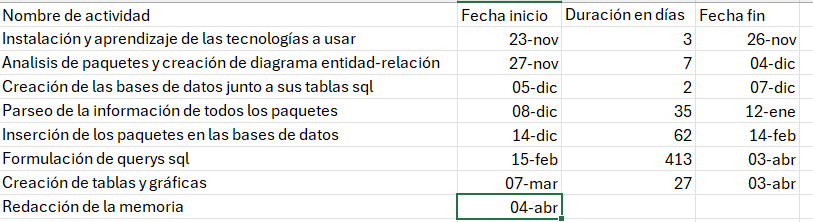
\includegraphics[width=9cm, keepaspectratio]{img/Gantt.png}
	\caption{Diagrama de Gantt}
	\label{fig:diagrama_gantt}
\end{figure}

%%%%%%%%%%%%%%%%%%%%%%%%%%%%%%%%%%%%%%%%%%%%%%%%%%%%%%%%%%%%%%%%%%%%%%%%%%%%%%%%
%%%%%%%%%%%%%%%%%%%%%%%%%%%%%%%%%%%%%%%%%%%%%%%%%%%%%%%%%%%%%%%%%%%%%%%%%%%%%%%%
% ESTADO DEL ARTE %
%%%%%%%%%%%%%%%%%%%%%%%%%%%%%%%%%%%%%%%%%%%%%%%%%%%%%%%%%%%%%%%%%%%%%%%%%%%%%%%%

\cleardoublepage
\chapter{Estado del arte}
\label{chap:estado}


\section{Python 3.12.0} 
\label{sec:python}
\textbf{Python}~\cite{oracle:_python} es un lenguaje de programación orientado a objetos de alto nivel con una sintaxis fácil de interpretar y leer. Tiene un amplio uso en computación científica, desarrollo web y automatización.

\textbf{Peter Norvig}, director de investigación de Google afirma que "Python ha sido una parte importante de Google desde el principio, y permanece así a medida que el sistema crece y evoluciona".

Al ser un lenguaje popular tiene una mayor selección de bibliotecas, lo que ahorra a un desarrollador cantidades increíbles de tiempo y esfuerzo. También tiene más tutoriales y documentación. Esto aumenta las probabilidades de encontrar soluciones a los problemas.

Una curiosidad del lenguaje es que la empresa de mayor emprendimiento de la "inteligencia artificial"  \textbf{ Open AI\footnote{\url{https://platform.openai.com/docs/libraries/python-library}}} está diseñada con python en gran parte y sus bibliotecas son públicas para su uso.

En la figura~\ref{fig:evolucion_python} podemos observar que Python es el lenguaje más usado del mundo según sus últimos datos en 2019~\cite{statista:_tecnología}.

\begin{figure}
	\centering
	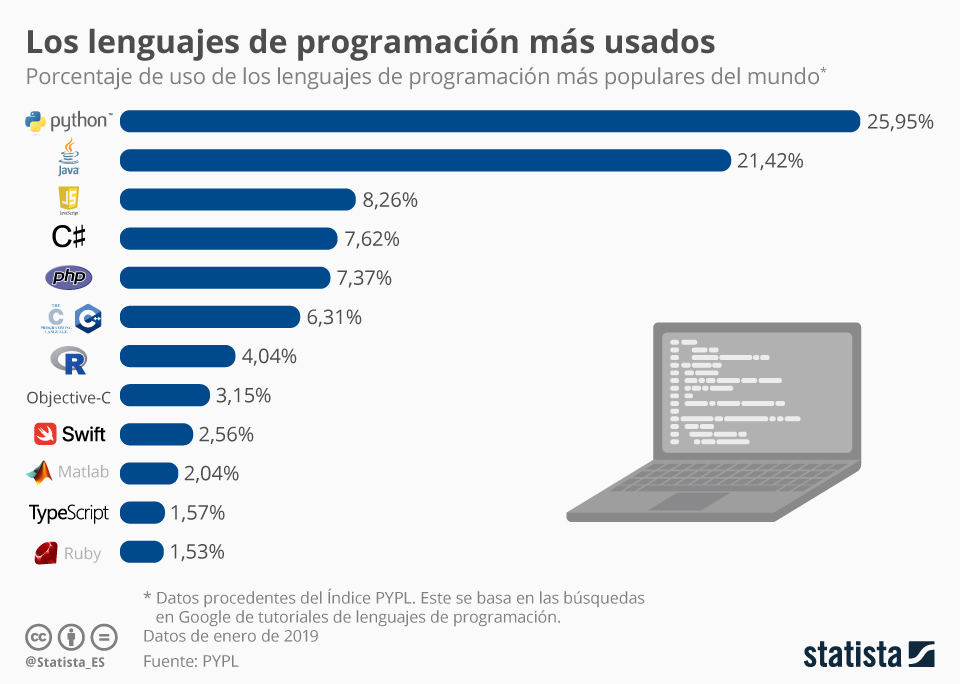
\includegraphics[width=14cm, keepaspectratio]{img/ev_python.jpeg}
	\caption{Lenguajes de programación más populares del mundo}
	\label{fig:evolucion_python}
\end{figure}

\section{My sql connector} 
\label{sec:mysqlconnector}
Esta es la librería más importante de Python para poder desarrollar este proyecto.
MySQL Connector/Python~\cite{mysql:_connectors} permite a los programas de Python acceder a las bases de datos MySQL, utilizando una API que cumple con la Especificación de API de Base de Datos de Python.
Sus funciones más destacadas e importantes son:
\begin{enumerate}
	\item \textbf{Conexión a la base de datos: }con la función \textbf{mysql.connector.connect().}
	\item \textbf{Ejecución de consultas SQL: }con la función \textbf{cursor.execute().}
	\item \textbf{Recuperación de resultados: }con la función \textbf{cursor.fetchall()}.
	\item \textbf{Inserción, actualización y eliminación de datos: }con consultas SQL como INSERT, UPDATE y DELETE, ejecutadas con la función \textbf{cursor.execute().}
	\item \textbf{Gestión de errores: }se capturan y manejan errores en el código Python usando excepciones.
	\item \textbf{Desconexión de la base de datos: }con la función \textbf{connection.close().}
\end{enumerate}

\section{Matplotlib} 
\label{sec:Matplotlib}


Matplotlibes~\cite{python:_matplotlib} es una librería de Python open source. John Hunter, neurobiólogo, fue su desarrollador inicial en 2002. Su objetivo era visualizar las señales eléctricas del cerebro de personas epilépticas. Por ello intentó replicar las diferentes funcionalidades de MATLAB (gráficas) con Python. 

Matplotlib ha sido mejorado a lo largo del tiempo por numerosos contribuidores de la comunidad open source. Se usa para crear gráficas y diagramas de gran calidad que aportan la visualización de los datos de  forma detallada.

Es posible crear trazados, histogramas, diagramas de barras y cualquier tipo de gráfica como en la Figura ~\ref{fig:matplotlib} con unas lineas de código.

Esta librería es particularmente útil para las personas que trabajan con Python o NumPy.

\begin{figure}
	\centering
	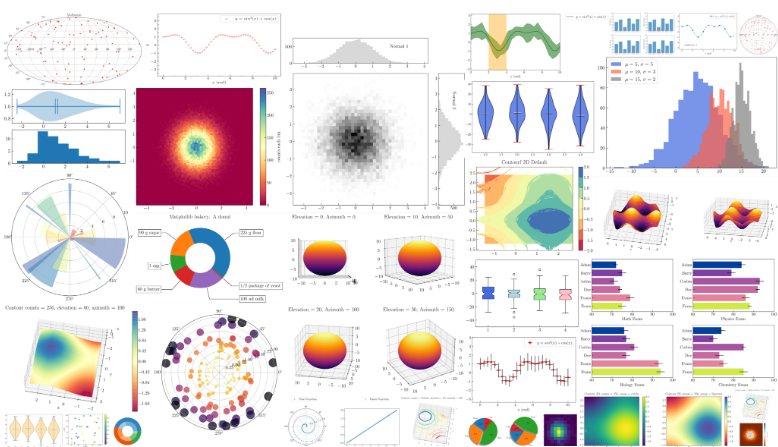
\includegraphics[width=14cm, keepaspectratio]{img/Matplotlib.png}
	\caption{Ejemplos gráficas Matplotlib}
	\label{fig:matplotlib}
\end{figure}
%%%%%%%%%%%%%%%%%%%%%%%%%%%%%%%%%%%%%%%%%%%%%%%%%%%%%%%%%%%%%%%%%%%%%%%%%%%%%%%%
%%%%%%%%%%%%%%%%%%%%%%%%%%%%%%%%%%%%%%%%%%%%%%%%%%%%%%%%%%%%%%%%%%%%%%%%%%%%%%%%
% DISEÑO E IMPLEMENTACIÓN %
%%%%%%%%%%%%%%%%%%%%%%%%%%%%%%%%%%%%%%%%%%%%%%%%%%%%%%%%%%%%%%%%%%%%%%%%%%%%%%%%

\cleardoublepage
\chapter{Diseño e implementación}
\label{sec:diseno}

Aquí viene todo lo que has hecho tú (tecnológicamente). 
Puedes entrar hasta el detalle. 
Es la parte más importante de la memoria, porque describe lo que has hecho tú.
Eso sí, normalmente aconsejo no poner código, sino diagramas.



\section{Arquitectura general} 
\label{sec:arquitectura}

Si tu proyecto es un software, siempre es bueno poner la arquitectura (que es cómo se estructura tu programa a ``vista de pájaro'').

\begin{figure}
  \centering
  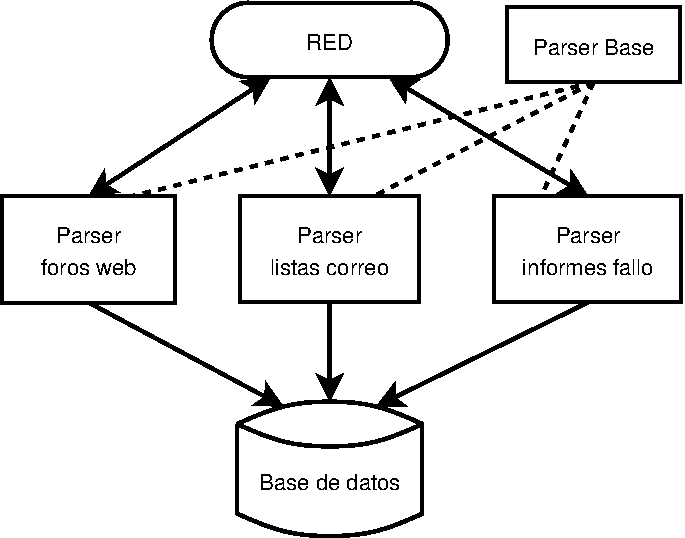
\includegraphics[width=9cm, keepaspectratio]{img/arquitectura.png}
  \caption{Estructura del parser básico}
  \label{fig:arquitectura}
\end{figure}


Por ejemplo, puedes verlo en la figura~\ref{fig:arquitectura}.
\LaTeX \ pone las figuras donde mejor cuadran. 
Y eso quiere decir que quizás no lo haga donde lo hemos puesto\ldots 
Eso no es malo.
A veces queda un poco raro, pero es la filosofía de \LaTeX: tú al contenido, que yo me encargo de la maquetación.


 
Recuerda que toda figura que añadas a tu memoria debe ser explicada.
Sí, aunque te parezca evidente lo que se ve en la figura~\ref{fig:arquitectura}, la figura en sí solamente es un apoyo a tu texto.
Así que explica lo que se ve en la figura, haciendo referencia a la misma tal y como ves aquí.
Por ejemplo: En la figura~\ref{fig:arquitectura} se puede ver que la estructura del \emph{parser} básico, que consta de seis componentes diferentes: los datos se obtienen de la red, y según el tipo de dato, se pasará a un \emph{parser} específico y bla, bla, bla\ldots

Si utilizas una base de datos, no te olvides de incluir también un diagrama de entidad-relación.


%%%%%%%%%%%%%%%%%%%%%%%%%%%%%%%%%%%%%%%%%%%%%%%%%%%%%%%%%%%%%%%%%%%%%%%%%%%%%%%%
%%%%%%%%%%%%%%%%%%%%%%%%%%%%%%%%%%%%%%%%%%%%%%%%%%%%%%%%%%%%%%%%%%%%%%%%%%%%%%%%
% EXPERIMENTOS Y VALIDACIÓN %
%%%%%%%%%%%%%%%%%%%%%%%%%%%%%%%%%%%%%%%%%%%%%%%%%%%%%%%%%%%%%%%%%%%%%%%%%%%%%%%%

\cleardoublepage
\chapter{Experimentos y validación}
\label{chap:experimentos}

Este capítulo se introdujo como requisito en 2019. 
Describe los experimentos y casos de test que tuviste que implementar para validar tus resultados. 
Incluye también los resultados de validación que permiten afirmar que tus resultados son correctos. 


%%%%%%%%%%%%%%%%%%%%%%%%%%%%%%%%%%%%%%%%%%%%%%%%%%%%%%%%%%%%%%%%%%%%%%%%%%%%%%%%
%%%%%%%%%%%%%%%%%%%%%%%%%%%%%%%%%%%%%%%%%%%%%%%%%%%%%%%%%%%%%%%%%%%%%%%%%%%%%%%%
% RESULTADOS %
%%%%%%%%%%%%%%%%%%%%%%%%%%%%%%%%%%%%%%%%%%%%%%%%%%%%%%%%%%%%%%%%%%%%%%%%%%%%%%%%

\cleardoublepage
\chapter{Resultados}
\label{chap:resultados}

En este capítulo se incluyen los resultados de tu trabajo fin de grado.

Si es una herramienta de análisis lo que has realizado, aquí puedes poner ejemplos de haberla utilizado para que se vea su utilidad.


%%%%%%%%%%%%%%%%%%%%%%%%%%%%%%%%%%%%%%%%%%%%%%%%%%%%%%%%%%%%%%%%%%%%%%%%%%%%%%%%
%%%%%%%%%%%%%%%%%%%%%%%%%%%%%%%%%%%%%%%%%%%%%%%%%%%%%%%%%%%%%%%%%%%%%%%%%%%%%%%%
% CONCLUSIONES %
%%%%%%%%%%%%%%%%%%%%%%%%%%%%%%%%%%%%%%%%%%%%%%%%%%%%%%%%%%%%%%%%%%%%%%%%%%%%%%%%

\cleardoublepage
\chapter{Conclusiones}
\label{chap:conclusiones}


\section{Consecución de objetivos}
\label{sec:consecucion-objetivos}

Esta sección es la sección espejo de las dos primeras del capítulo de objetivos, donde se planteaba el objetivo general y se elaboraban los específicos.

Es aquí donde hay que debatir qué se ha conseguido y qué no. 
Cuando algo no se ha conseguido, se ha de justificar, en términos de qué problemas se han encontrado y qué medidas se han tomado para mitigar esos problemas.

Y si has llegado hasta aquí, siempre es bueno pasarle el corrector ortográfico, que las erratas quedan fatal en la memoria final.
Para eso, en Linux tenemos aspell, que se ejecuta de la siguiente manera desde la línea de \emph{shell}:

\begin{verbatim}
  aspell --lang=es_ES -c memoria.tex
\end{verbatim}

\section{Aplicación de lo aprendido}
\label{sec:aplicacion}

Aquí viene lo que has aprendido durante el Grado/Máster y que has aplicado en el TFG/TFM.
Una buena idea es poner las asignaturas más relacionadas y comentar en un párrafo los conocimientos y habilidades puestos en práctica.

\begin{enumerate}
  \item a
  \item b
\end{enumerate}


\section{Lecciones aprendidas}
\label{sec:lecciones_aprendidas}

Aquí viene lo que has aprendido en el Trabajo Fin de Grado/Máster.

\begin{enumerate}
  \item Aquí viene uno.
  \item Aquí viene otro.
\end{enumerate}


\section{Trabajos futuros}
\label{sec:trabajos_futuros}

Ningún proyecto ni software se termina, así que aquí vienen ideas y funcionalidades que estaría bien tener implementadas en el futuro.

Es un apartado que sirve para dar ideas de cara a futuros TFGs/TFMs.


%%%%%%%%%%%%%%%%%%%%%%%%%%%%%%%%%%%%%%%%%%%%%%%%%%%%%%%%%%%%%%%%%%%%%%%%%%%%%%%%
%%%%%%%%%%%%%%%%%%%%%%%%%%%%%%%%%%%%%%%%%%%%%%%%%%%%%%%%%%%%%%%%%%%%%%%%%%%%%%%%
% APÉNDICE(S) %
%%%%%%%%%%%%%%%%%%%%%%%%%%%%%%%%%%%%%%%%%%%%%%%%%%%%%%%%%%%%%%%%%%%%%%%%%%%%%%%%

\cleardoublepage
\appendix
\chapter{Manual de usuario}
\label{app:manual}

Esto es un apéndice.
Si has creado una aplicación, siempre viene bien tener un manual de usuario.
Pues ponlo aquí.

%%%%%%%%%%%%%%%%%%%%%%%%%%%%%%%%%%%%%%%%%%%%%%%%%%%%%%%%%%%%%%%%%%%%%%%%%%%%%%%%
%%%%%%%%%%%%%%%%%%%%%%%%%%%%%%%%%%%%%%%%%%%%%%%%%%%%%%%%%%%%%%%%%%%%%%%%%%%%%%%%
% BIBLIOGRAFIA %
%%%%%%%%%%%%%%%%%%%%%%%%%%%%%%%%%%%%%%%%%%%%%%%%%%%%%%%%%%%%%%%%%%%%%%%%%%%%%%%%

\cleardoublepage

% Las siguientes dos instrucciones es todo lo que necesitas
% para incluir las citas en la memoria
\bibliographystyle{abbrv}
\bibliography{memoria}  % memoria.bib es el nombre del fichero que contiene
% las referencias bibliográficas. Abre ese fichero y mira el formato que tiene,
% que se conoce como BibTeX. Hay muchos sitios que exportan referencias en
% formato BibTeX. Prueba a buscar en http://scholar.google.com por referencias
% y verás que lo puedes hacer de manera sencilla.
% Más información: 
% http://texblog.org/2014/04/22/using-google-scholar-to-download-bibtex-citations/

\end{document}
